Att exekvera ett program symboliskt innebär att representera värden utefter 
programflödet som symboliska restriktioner (jfr en. constraint), vilka kan lösas av automatiserade 
teoremlösare (\emph{SMT solver}). En symbolisk körning representerar flera konkreta 
körningar eftersom de (symboliska) värden som används representerar grupper av 
konkreta värden vilka har gemensamt hur de påverkar programmets flöde. 

Vägar i programmets kontrollflöde utforskas med symboliska uttryck som kallas
för path constraint (jfr sv. vägvillkor) för de begränsningar som finns på
programmets variabler -- vilka egenskaper de måste uppnå för att just denna väg
ska kunna följas. Eftersom de symboliska värdena har kapacitet att representera
grupperingar av konkreta värden istället för enskilda sådana, utförs en
generaliserad testning av programmet, som ger insikt i hur programmet beter sig
givet en grupp av parametrar som alla på grund av någon eller några gemensamma
egenskaper, orsakar gemensamma beteenden i programmet. 

En symbolisk exekveringsmotor arbetar genom att först representera programmets
input som symboliska variablar, vilka vid starten inte har några begränsningar,
och när programflödet når en branch som baseras på någon av de symboliska
variablerna, väljer motorn en branch och tillsätter dess path constraint på den
symboliska variabeln för alla vägar som fortsätter utefter branchen. Operationer
på värden under körningens väg översätts till symboliska operationer på
motsvarande symboliska variabler \cite{klee}. När körning utefter branchen är
slutförd repeterar motorn samma metodik på samma branch för att utforska andra
alternativ. De tillståndsvillkor som en viss väg visas ha byggs därför
successivt upp genom att motorn utökar de symboliska variablerna till
villkorliga uttryck allt eftersom vägen följs. 

De fel som hittas genom symbolisk exekvering är tillförlitliga då metoden ej ger falskt 
positiva resultat. Huruvida villkorsblock av program är nårbara kan evalueras med 
säkerhet eftersom de krav som måste uppfyllas för att följa vägen dit dokumenteras under 
den symboliska körningen, och resulterar i fullständiga symboliska representationer 
som en automatiserad teoremlösare (SMT solver) kan appliceras på. 

Symbolisk exekvering är användbart för att resonera kring hur programmet beter sig 
beroende på grupperingar av input. För program där få värden tar gemensamma vägar blir 
fördelen försumbar av att använda dynamisk testning av konkret data. 

Eftersom symbolisk exekvering kan leda till \emph{path explosion}, vilket
uppstår i program vars branches växer exponentiellt och resulterar i att en
symbolisk exekvering aldrig terminerar \cite{path_explo}, är det inte effektivt 
att alltid undersöka alla branchar i ett program. Exempel på metoder för att undvika 
path explosion är \emph{state-merging} och \emph{heuristics}. 

För att illustrera symbolisk exekvering används följande pseudokod:

\begin{figure}[H]
\centering
\begin{lstlisting}[label={list:first}, language=Python, frame=single]
x = int(argv[1])
y = int(argv[2])
z = 2 * y

if x == 100000: 
  if x < z:
  // fabricated scenario of 
  // memory vulnerability
    error_leading_to_mem_vuln()
  else:
    run_other_important_code()
else:
  run_important_code()

\end{lstlisting}
\caption{}
\end{figure}

Exemplet ovan använder symbolisk exekvering för att hitta vilken input som leder
till de olika vägarna. I många fall är det intressant att göra en uttömmande
sökning och hitta alla möjliga vägar i ett program, något som är möjligt i detta
program men inte alla program. Variablerna x och y sätts till symboliska
värden som sedan används för att beräkna path constraint och de symboliska
uttryck som variablerna utvecklas till för en vald branch. Därefter används
dessa uttryck och path constraint tillsammans för att bilda en ekvation som kan
lösas med hjälp av en SMT-solver och därmed få ut ett konkret värde. Figur 2.4
visar hur det symboliska tillståndet förändras för alla möjliga branches i
programmet.

\begin{figure}[H]
\centering
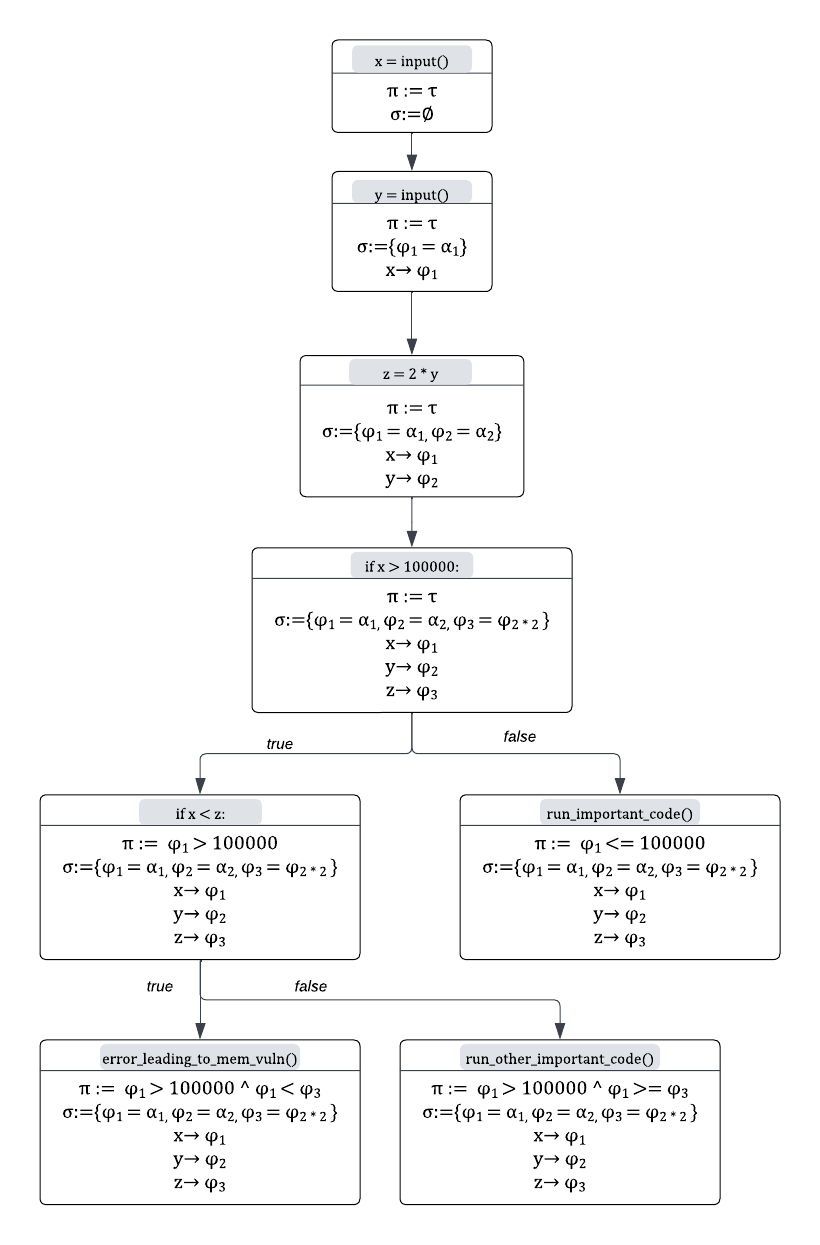
\includegraphics[scale=0.5]{figures/final_symbolic_example_graph.png}
\caption{Path constraint och symboliskt tillstånd för alla vägar i
    pseudokoden angett i figur 2.3.}
\end{figure}

I figuren ovan används $\pi$ för att ange path constraint vilket är initialt satt
till $\top$ eftersom villkoret är sant från början och $\phi$ används för att visa
mappningen för symboliska värden.

